\chapter{Application: Modal Logic for AI Agents}

\begin{goals}
\begin{itemize}
    \item See how modal logic applies to AI agent design
    \item Understand the two-layer architecture
    \item Connect PDL to agent planning
    \item Appreciate the synthesis: logic + learning
\end{itemize}
\end{goals}

\section{The Problem with Current Agents}

LLM-based agents (ReAct, CoT, Tool Use) are:
\begin{itemize}
    \item Engineering patchwork, no theoretical foundation
    \item Hard to verify or constrain
    \item Essentially automata, but not formalized as such
\end{itemize}

\begin{warning}
Current agent frameworks rediscover automata theory and modal logic concepts, but without the rigor. We can do better.
\end{warning}

\section{The Two-Layer Architecture}

\begin{center}
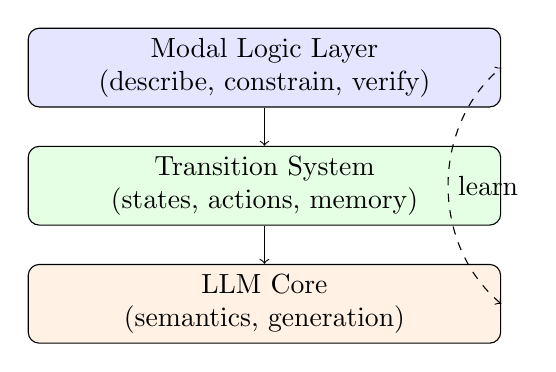
\begin{tikzpicture}[
    box/.style={draw, rounded corners, minimum width=6cm, minimum height=1cm, align=center}
]
\node[box, fill=blue!10] (logic) at (0,3) {Modal Logic Layer\\(describe, constrain, verify)};
\node[box, fill=green!10] (trans) at (0,1.5) {Transition System\\(states, actions, memory)};
\node[box, fill=orange!10] (llm) at (0,0) {LLM Core\\(semantics, generation)};

\draw[->] (logic) -- (trans);
\draw[->] (trans) -- (llm);
\draw[<->, dashed] (llm.east) to[bend left=50] node[right] {learn} (logic.east);
\end{tikzpicture}
\end{center}

\textbf{Modal Logic Layer}: Specify constraints, verify properties

\textbf{Transition System}: Concrete state machine (coalgebra!)

\textbf{LLM Core}: Handle natural language, generate content

\section{PDL for Agent Actions}

Agent capabilities as atomic actions:
\begin{itemize}
    \item $\mathsf{search}$ — search the web
    \item $\mathsf{compute}$ — run calculation
    \item $\mathsf{ask}$ — query user
    \item $\mathsf{store}$, $\mathsf{retrieve}$ — memory operations
\end{itemize}

Complex behaviors as PDL programs:
\begin{align*}
&[\mathsf{search};\mathsf{summarize}]\mathsf{hasAnswer} \\
&\quad \text{``search then summarize guarantees an answer''} \\[1em]
&\langle(\mathsf{try}_1 \cup \mathsf{try}_2 \cup \mathsf{try}_3)\rangle\mathsf{success} \\
&\quad \text{``one of three attempts can succeed''}
\end{align*}

\section{Relevant Modal Logics}

\begin{center}
\begin{tabular}{ll}
\textbf{Logic} & \textbf{Agent Application} \\
\hline
Epistemic ($K_a\varphi$) & ``Agent knows $\varphi$'' \\
Deontic ($O\varphi$, $P\varphi$) & ``Agent must/may do $\varphi$'' \\
PDL ($[\alpha]\varphi$) & ``After action $\alpha$, $\varphi$ holds'' \\
Temporal (LTL/CTL) & ``Eventually goal'', ``Always safe'' \\
Graded ($\possible_{\geq n}\varphi$) & ``At least $n$ options available'' \\
\end{tabular}
\end{center}

\section{The Synthesis}

\textbf{From logic}: precision, verifiability, constraints

\textbf{From learning}: adaptability, learning from data

\textbf{Combined}:
\begin{enumerate}
    \item Specify agent behavior in modal logic
    \item Use semiring-valued coalgebra for soft version
    \item Train via gradient descent
    \item Extract crisp transition system
    \item Verify against modal specifications
\end{enumerate}

\begin{example}[Safe Agent]
Specification: ``Always have at least 2 safe actions available.''
\[
\mathsf{AG}\,(\possible_{\geq 2}\mathsf{safe})
\]

Train soft model → converge to crisp → verify specification holds.
\end{example}

\section{Learning Modal Abstractions}

Key insight: don't expose raw memory/tape to reasoning.

Instead, abstract into modal operators:
\begin{align*}
\necessary_{\mathsf{memory}}\varphi &\quad \text{``everything in memory satisfies $\varphi$''} \\
\possible_{\mathsf{action}}\mathsf{goal} &\quad \text{``some action can reach goal''}
\end{align*}

The agent reasons at the modal level. The transition system implements it.

\begin{keyinsight}
Modal logic provides the \emph{specification language} for agents. Coalgebra provides the \emph{implementation structure}. Semiring learning provides the \emph{training method}. Together: learnable, verifiable agents.
\end{keyinsight}

\section{Open Problems}

\begin{enumerate}
    \item How to automatically translate natural language goals to modal formulas?
    \item How to handle uncertainty? (Probabilistic modal logic)
    \item How to learn the right modal abstractions?
    \item Scalability to real-world agent complexity?
\end{enumerate}
